\documentclass[aspectratio=169,14pt]{beamer}

% Theme and styling
\usetheme{Madrid}
\usecolortheme{whale}
\setbeamertemplate{navigation symbols}{}
\setbeamertemplate{footline}[frame number]

% LARGER FONTS for projector
\setbeamerfont{title}{size=\Huge}
\setbeamerfont{frametitle}{size=\LARGE}
\setbeamerfont{block title}{size=\large}

% Packages
\usepackage{amsmath,amssymb,amsfonts}
\usepackage{graphicx}
\usepackage{xcolor}
\usepackage{tikz}
\usetikzlibrary{arrows.meta,positioning,shapes.geometric}
\usepackage{hyperref}
\usepackage{booktabs}

% Custom colors
\definecolor{chaosblue}{RGB}{25,84,123}
\definecolor{attractorred}{RGB}{180,40,40}
\definecolor{limitgreen}{RGB}{34,139,34}
\definecolor{caborange}{RGB}{230,120,20}

% Set paths
\graphicspath{{media/images/}}

% Title information
\title[Dynamical Systems]{Strange Attractors \& Dynamical Systems}
\subtitle{From Van der Pol Oscillators to Deterministic Chaos}
\author{Dynamical Systems Exploration}
\date{\today}
\institute{Mathematical Physics}

\begin{document}

%=============================================================================
% TITLE SLIDE
%=============================================================================
\begin{frame}
    \titlepage
\end{frame}

%=============================================================================
% TABLE OF CONTENTS
%=============================================================================
\begin{frame}{Outline}
    \tableofcontents
\end{frame}

%=============================================================================
% SECTION 1: WHAT ARE STRANGE ATTRACTORS?
%=============================================================================
\section{What Are Strange Attractors?}

\begin{frame}{The Nature of Dynamical Systems}
    \begin{columns}
        \begin{column}{0.45\textwidth}
            \textbf{\Large Key Question:}\\[0.8em]
            What happens to systems over long time periods?
            
            \vspace{1.2em}
            \textbf{Attractors} are the geometric structures toward which dynamical systems evolve.
            
            \vspace{1.2em}
            \begin{itemize}
                \item \textcolor{chaosblue}{\textbf{Fixed points}} (stable equilibria)
                \item \textcolor{limitgreen}{\textbf{Limit cycles}} (periodic orbits)
                \item \textcolor{attractorred}{\textbf{Strange attractors}} (chaos)
            \end{itemize}
        \end{column}
        \begin{column}{0.55\textwidth}
            \centering
            \includegraphics[width=\textwidth]{grand_comparison.png}
        \end{column}
    \end{columns}
\end{frame}

\begin{frame}{From Order to Chaos}
    \begin{block}{\Large The Lyapunov Exponent}
        Measures the rate of separation of infinitesimally close trajectories:
        \[
            \boxed{\Large |\delta\mathbf{x}(t)| \sim |\delta\mathbf{x}_0| \, e^{\lambda t}}
        \]
    \end{block}
    
    \vspace{1.5em}
    \begin{columns}
        \begin{column}{0.5\textwidth}
            \Large
            \begin{itemize}
                \item $\lambda < 0$: \textbf{Stable}
                \item $\lambda = 0$: Marginally stable
                \item $\lambda > 0$: \textcolor{attractorred}{\textbf{Chaotic!}}
            \end{itemize}
        \end{column}
        \begin{column}{0.5\textwidth}
            \begin{alertblock}{\large Deterministic Chaos}
                Simple equations can produce \textbf{unpredictable} behavior!
            \end{alertblock}
        \end{column}
    \end{columns}
\end{frame}

%=============================================================================
% SECTION 2: VAN DER POL OSCILLATOR
%=============================================================================
\section{Van der Pol Oscillator}

\begin{frame}{The Van der Pol Equation}
    \begin{block}{\Large Governing Equation (1927)}
        \[
            \boxed{\Large \frac{d^2x}{dt^2} - \mu(1-x^2)\frac{dx}{dt} + x = 0}
        \]
    \end{block}
    
    \vspace{0.8em}
    \textbf{\large First-order system form:}
    \[
        \Large
        \begin{cases}
            \dot{x} = y \\[0.5em]
            \dot{y} = \mu(1-x^2)y - x
        \end{cases}
    \]
    
    \vspace{0.5em}
    \begin{columns}
        \begin{column}{0.5\textwidth}
            \begin{itemize}
                \item $\mu > 0$: Nonlinear damping
                \item Discovered in vacuum tubes
                \item First example of \textbf{limit cycle}
            \end{itemize}
        \end{column}
        \begin{column}{0.5\textwidth}
            \begin{alertblock}{\large Key Feature}
                Amplitude-dependent damping creates \textbf{self-sustained oscillations}
            \end{alertblock}
        \end{column}
    \end{columns}
\end{frame}

\begin{frame}{Energy Pumping Mechanism}
    \begin{columns}
        \begin{column}{0.5\textwidth}
            \textbf{\large Effective damping coefficient:}
            \[
                \Large \gamma_{\text{eff}}(x) = -\mu(1 - x^2)
            \]
            
            \vspace{0.8em}
            \large
            \begin{tabular}{|c|c|c|}
                \hline
                \textbf{Condition} & \textbf{Damping} & \textbf{Effect} \\
                \hline
                $|x| < 1$ & Negative & Energy IN \\
                $|x| = 1$ & Zero & Balance \\
                $|x| > 1$ & Positive & Energy OUT \\
                \hline
            \end{tabular}
            
            \vspace{0.8em}
            \textbf{Result:} Self-regulating limit cycle
        \end{column}
        \begin{column}{0.5\textwidth}
            \centering
            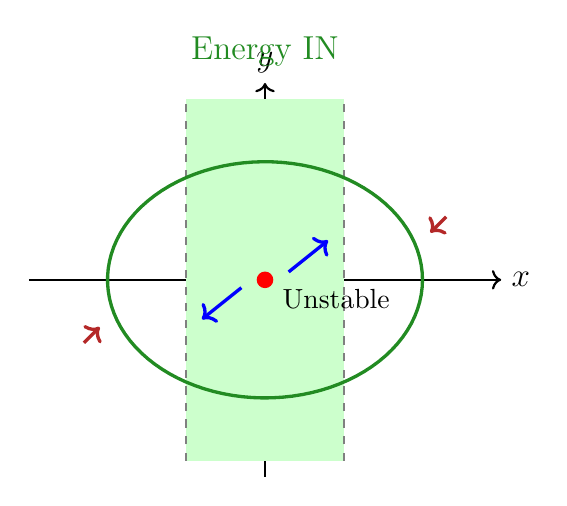
\begin{tikzpicture}[scale=1.0]
                \draw[->,thick] (-3,0) -- (3,0) node[right] {\large $x$};
                \draw[->,thick] (0,-2.5) -- (0,2.5) node[above] {\large $y$};
                % Energy zones
                \fill[green!20] (-1,-2.3) rectangle (1,2.3);
                \draw[dashed,gray,thick] (-1,-2.3) -- (-1,2.3);
                \draw[dashed,gray,thick] (1,-2.3) -- (1,2.3);
                % Limit cycle
                \draw[very thick,limitgreen,domain=0:360,samples=100] 
                    plot ({2*cos(\x)},{1.5*sin(\x)});
                % Arrows showing dynamics
                \draw[->,blue,very thick] (0.3,0.1) -- (0.8,0.5);
                \draw[->,blue,very thick] (-0.3,-0.1) -- (-0.8,-0.5);
                \draw[->,attractorred,very thick] (2.3,0.8) -- (2.1,0.6);
                \draw[->,attractorred,very thick] (-2.3,-0.8) -- (-2.1,-0.6);
                % Labels
                \node at (0,2.9) {\large\textcolor{limitgreen}{Energy IN}};
                \fill[red] (0,0) circle (3pt);
                \node[below right] at (0.1,0) {Unstable};
            \end{tikzpicture}
        \end{column}
    \end{columns}
\end{frame}

\begin{frame}{Phase Plane Analysis: Nullclines}
    \begin{columns}
        \begin{column}{0.5\textwidth}
            \textbf{Nullclines} are curves where $\dot{x} = 0$ or $\dot{y} = 0$:
            
            \vspace{0.5em}
            \textbf{$x$-nullcline} ($\dot{x} = 0$):
            \[
                y = 0 \quad \text{(the $x$-axis)}
            \]
            
            \textbf{$y$-nullcline} ($\dot{y} = 0$):
            \[
                y = \frac{x}{\mu(1-x^2)}
            \]
            
            \vspace{0.5em}
            \textbf{Equilibria} occur at nullcline intersections.
            
            \vspace{0.3em}
            Only one equilibrium: \textcolor{attractorred}{$(0, 0)$}
        \end{column}
        \begin{column}{0.5\textwidth}
            \centering
            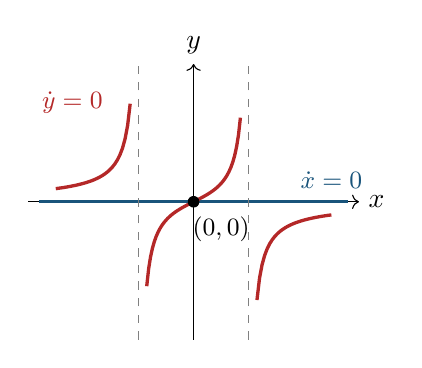
\begin{tikzpicture}[scale=0.7]
                \draw[->] (-3,0) -- (3,0) node[right] {$x$};
                \draw[->] (0,-2.5) -- (0,2.5) node[above] {$y$};
                % x-nullcline (y=0)
                \draw[very thick,chaosblue] (-2.8,0) -- (2.8,0);
                \node[chaosblue] at (2.5,0.4) {\small $\dot{x}=0$};
                % y-nullcline (cubic-like curve)
                \draw[very thick,attractorred,domain=-0.85:0.85,samples=50] 
                    plot (\x, {0.5*\x/(1-\x*\x)});
                \draw[very thick,attractorred,domain=-2.5:-1.15,samples=30] 
                    plot (\x, {0.5*\x/(1-\x*\x)});
                \draw[very thick,attractorred,domain=1.15:2.5,samples=30] 
                    plot (\x, {0.5*\x/(1-\x*\x)});
                \node[attractorred] at (-2.2,1.8) {\small $\dot{y}=0$};
                % Equilibrium
                \fill[black] (0,0) circle (3pt);
                \node at (0.5,-0.5) {\small $(0,0)$};
                % Asymptotes
                \draw[dashed,gray] (-1,-2.5) -- (-1,2.5);
                \draw[dashed,gray] (1,-2.5) -- (1,2.5);
            \end{tikzpicture}
        \end{column}
    \end{columns}
\end{frame}

\begin{frame}{Equilibrium Analysis: The Jacobian Matrix}
    \begin{block}{\Large General Jacobian}
        For $\dot{x} = f(x,y)$, $\dot{y} = g(x,y)$:
        \[
            \Large J(x,y) = \begin{pmatrix}
                \frac{\partial f}{\partial x} & \frac{\partial f}{\partial y} \\[0.5em]
                \frac{\partial g}{\partial x} & \frac{\partial g}{\partial y}
            \end{pmatrix}
            = \begin{pmatrix}
                0 & 1 \\[0.3em]
                -2\mu xy - 1 & \mu(1-x^2)
            \end{pmatrix}
        \]
    \end{block}
    
    \vspace{1em}
    \textbf{\large At the origin} $(x, y) = (0, 0)$:
    \[
        \boxed{\Large J(0,0) = \begin{pmatrix}
            0 & 1 \\
            -1 & \mu
        \end{pmatrix}}
    \]
    
    \vspace{0.5em}
    \large
    \begin{itemize}
        \item Trace: $\text{tr}(J) = \mu > 0$ \quad (sum of eigenvalues)
        \item Determinant: $\det(J) = 1 > 0$ \quad (product of eigenvalues)
    \end{itemize}
\end{frame}

\begin{frame}{Eigenvalue Analysis: Stability Classification}
    \textbf{\Large Characteristic equation:} $\quad \lambda^2 - \mu\lambda + 1 = 0$
    
    \vspace{0.8em}
    \begin{block}{\Large Eigenvalues}
        \[
            \boxed{\Large \lambda_{1,2} = \frac{\mu \pm \sqrt{\mu^2 - 4}}{2}}
        \]
    \end{block}
    
    \vspace{0.5em}
    \textbf{\large Discriminant:} $\Delta = \mu^2 - 4$
    
    \vspace{0.8em}
    \begin{center}
    \large
    \begin{tabular}{|c|c|c|}
        \hline
        \textbf{$\mu$ range} & \textbf{Eigenvalues} & \textbf{Stability} \\
        \hline
        $\mu = 0$ & $\pm i$ & Neutral center \\
        \hline
        $0 < \mu < 2$ & Complex, Re $> 0$ & \textcolor{attractorred}{Unstable spiral} \\
        \hline
        $\mu \geq 2$ & Real, both $> 0$ & \textcolor{attractorred}{Unstable node} \\
        \hline
    \end{tabular}
    \end{center}
    
    \vspace{0.5em}
    \begin{alertblock}{\large Conclusion}
        For \textbf{any} $\mu > 0$: origin is unstable — trajectories escape outward!
    \end{alertblock}
\end{frame}

\begin{frame}{The Poincaré-Bendixson Theorem}
    \textbf{\Large Question:} If the origin is unstable, where do trajectories go?
    
    \vspace{0.8em}
    \begin{block}{\Large Poincaré-Bendixson Theorem}
        If a trajectory in $\mathbb{R}^2$ enters a closed, bounded region $R$ containing \textbf{no equilibria} and never leaves, then it must approach a \textbf{periodic orbit}.
    \end{block}
    
    \vspace{0.8em}
    \textbf{\large Application to Van der Pol:}
    \begin{enumerate}
        \item Origin is unstable $\Rightarrow$ trajectories spiral \textit{outward}
        \item Energy dissipation when $|x| > 1$ $\Rightarrow$ trajectories are \textit{bounded}
        \item Trajectories enter an annular region with no equilibria
        \item $\therefore$ A \textcolor{limitgreen}{\textbf{limit cycle}} must exist!
    \end{enumerate}
    
    \vspace{0.5em}
    \begin{exampleblock}{\large Key Insight}
        The limit cycle is the \textit{unique} stable attractor for $\mu > 0$
    \end{exampleblock}
\end{frame}

\begin{frame}{Relaxation Oscillations: Large $\mu$}
    \begin{columns}
        \begin{column}{0.5\textwidth}
            When $\mu \gg 1$, the system exhibits \textbf{relaxation oscillations}:
            
            \vspace{0.5em}
            \begin{enumerate}
                \item \textbf{Slow phase:} Trajectory creeps along the cubic nullcline
                \item \textbf{Fast phase:} Rapid jump between branches
            \end{enumerate}
            
            \vspace{0.5em}
            \textbf{Period scaling:}
            \[
                T \approx (3 - 2\ln 2)\mu \approx 1.614\mu
            \]
            
            \vspace{0.3em}
            \textbf{Biological examples:}
            \begin{itemize}
                \item Heartbeat (SA node)
                \item Neural action potentials
                \item Predator-prey cycles
            \end{itemize}
        \end{column}
        \begin{column}{0.5\textwidth}
            \centering
            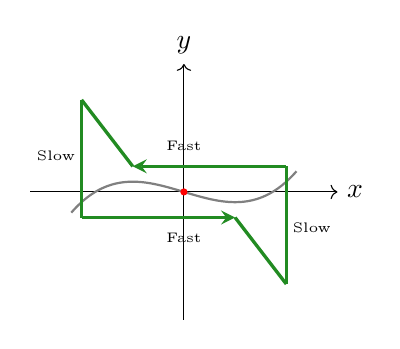
\begin{tikzpicture}[scale=0.65]
                \draw[->] (-3,0) -- (3,0) node[right] {$x$};
                \draw[->] (0,-2.5) -- (0,2.5) node[above] {$y$};
                % Cubic nullcline
                \draw[thick,gray,domain=-2.2:2.2,samples=100] 
                    plot (\x, {0.3*(\x*\x*\x/3 - \x)});
                % Relaxation cycle
                \draw[very thick,limitgreen] (-2,1.8) -- (-2,-0.5);
                \draw[very thick,limitgreen,->,>=stealth] (-2,-0.5) -- (1,-0.5);
                \draw[very thick,limitgreen] (2,-1.8) -- (2,0.5);
                \draw[very thick,limitgreen,->,>=stealth] (2,0.5) -- (-1,0.5);
                \draw[very thick,limitgreen] (-2,1.8) -- (-1,0.5);
                \draw[very thick,limitgreen] (2,-1.8) -- (1,-0.5);
                % Labels
                \node at (-2.5,0.7) {\tiny Slow};
                \node at (0,-0.9) {\tiny Fast};
                \node at (2.5,-0.7) {\tiny Slow};
                \node at (0,0.9) {\tiny Fast};
                \fill[red] (0,0) circle (2pt);
            \end{tikzpicture}
            
            \vspace{0.3em}
            \small Relaxation oscillation for $\mu \gg 1$
        \end{column}
    \end{columns}
\end{frame}

\begin{frame}{Heartbeat Modeling with Van der Pol}
    \begin{columns}
        \begin{column}{0.5\textwidth}
            The Van der Pol oscillator models \textbf{cardiac rhythms}:
            
            \vspace{0.5em}
            \begin{itemize}
                \item Sinoatrial node acts as a \textit{relaxation oscillator}
                \item Self-sustaining periodic signal
                \item Robust against perturbations
            \end{itemize}
            
            \vspace{0.5em}
            \begin{block}{FitzHugh-Nagumo Model}
                \[
                    \begin{cases}
                        \dot{v} = v - \frac{v^3}{3} - w + I_{\text{ext}} \\[0.3em]
                        \dot{w} = \epsilon(v + a - bw)
                    \end{cases}
                \]
            \end{block}
            
            \vspace{0.3em}
            \small A simplified Hodgkin-Huxley model
        \end{column}
        \begin{column}{0.5\textwidth}
            \textbf{Clinical connections:}
            
            \vspace{0.5em}
            \begin{tabular}{|l|l|}
                \hline
                \textbf{Normal} & Stable limit cycle \\
                & (60-100 bpm) \\
                \hline
                \textbf{Arrhythmia} & Bifurcation from \\
                & healthy cycle \\
                \hline
                \textbf{Pacemaker} & Artificial periodic \\
                & forcing \\
                \hline
            \end{tabular}
            
            \vspace{0.5em}
            \centering
            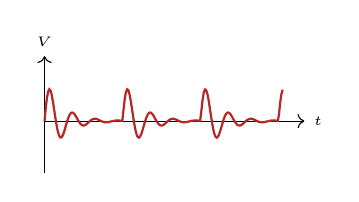
\begin{tikzpicture}[scale=0.55]
                \draw[->] (0,0) -- (6,0) node[right] {\tiny $t$};
                \draw[->] (0,-1.2) -- (0,1.5) node[above] {\tiny $V$};
                % Heartbeat waveform
                \draw[thick,attractorred,domain=0:5.5,samples=200] 
                    plot (\x, {1.0*exp(-2.5*mod(\x,1.8))*sin(12*mod(\x,1.8) r)});
            \end{tikzpicture}
        \end{column}
    \end{columns}
\end{frame}

\begin{frame}{Summary: Van der Pol Dynamics}
    \begin{center}
    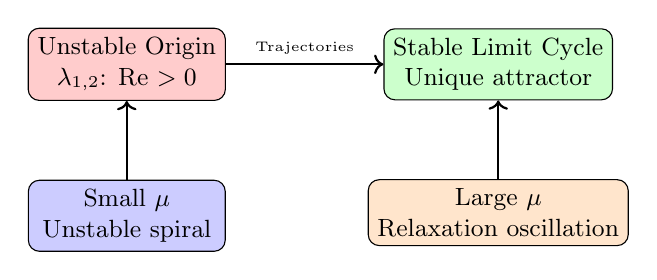
\begin{tikzpicture}[
        node distance=1.5cm,
        box/.style={rectangle, draw, rounded corners, minimum width=2.5cm, minimum height=0.8cm, align=center, font=\small}
    ]
        \node[box, fill=red!20] (origin) {Unstable Origin\\$\lambda_{1,2}$: Re $> 0$};
        \node[box, fill=green!20, right=2cm of origin] (limit) {Stable Limit Cycle\\Unique attractor};
        \node[box, fill=blue!20, below=1cm of origin] (small) {Small $\mu$\\Unstable spiral};
        \node[box, fill=orange!20, below=1cm of limit] (large) {Large $\mu$\\Relaxation oscillation};
        
        \draw[->,thick] (origin) -- (limit) node[midway,above] {\tiny Trajectories};
        \draw[->,thick] (small) -- (origin);
        \draw[->,thick] (large) -- (limit);
    \end{tikzpicture}
    \end{center}
    
    \vspace{0.5em}
    \begin{block}{Key Results}
        \begin{itemize}
            \item \textbf{Unique equilibrium} at origin — always unstable for $\mu > 0$
            \item \textbf{Limit cycle} guaranteed by Poincaré-Bendixson theorem
            \item \textbf{Applications:} Electronics, cardiology, neuroscience
        \end{itemize}
    \end{block}
\end{frame}

%=============================================================================
% SECTION 3: LORENZ SYSTEM
%=============================================================================
\section{The Lorenz System}

\begin{frame}{Lorenz Equations}
    \begin{block}{\Large The System (1963)}
        \[
            \boxed{\Large
            \begin{cases}
                \dot{x} = \sigma(y - x) \\[0.5em]
                \dot{y} = x(\rho - z) - y \\[0.5em]
                \dot{z} = xy - \beta z
            \end{cases}}
        \]
    \end{block}
    
    \vspace{1em}
    \textbf{\large Standard parameters:}
    \begin{itemize}
        \item $\sigma = 10$ (Prandtl number)
        \item $\rho = 28$ (Rayleigh number)
        \item $\beta = \frac{8}{3}$ (geometric factor)
    \end{itemize}
    
    \vspace{0.5em}
    \large Originally derived from atmospheric convection—now the \textbf{icon of chaos theory}.
\end{frame}

\begin{frame}{The Butterfly Attractor}
    \centering
    \includegraphics[width=0.92\textwidth]{lorenz_attractor_views.png}
    
    \vspace{0.5em}
    \large Four views of the Lorenz attractor revealing its intricate 3D structure
\end{frame}

\begin{frame}{Sensitive Dependence on Initial Conditions}
    \centering
    \includegraphics[width=0.95\textwidth]{butterfly_effect.png}
    
    \vspace{0.8em}
    \begin{quote}
        \Large ``Does the flap of a butterfly's wings in Brazil set off a tornado in Texas?''
        \hfill \normalsize — Edward Lorenz, 1972
    \end{quote}
\end{frame}

\begin{frame}{Fractal Structure of Strange Attractors}
    \begin{columns}
        \begin{column}{0.5\textwidth}
            \textbf{\large Properties:}
            \begin{itemize}
                \item Non-integer (fractal) dimension
                \item Lorenz attractor: $D \approx 2.06$
                \item Self-similar at all scales
                \item Infinite length, zero volume
            \end{itemize}
            
            \vspace{1.2em}
            \textbf{\large Lyapunov spectrum:}
            \begin{itemize}
                \item $\lambda_1 \approx +0.9$ (expansion)
                \item $\lambda_2 \approx 0$ (neutral)
                \item $\lambda_3 \approx -14.6$ (contraction)
            \end{itemize}
        \end{column}
        \begin{column}{0.5\textwidth}
            \centering
            \includegraphics[width=\textwidth]{poincare_section.png}
        \end{column}
    \end{columns}
\end{frame}

%=============================================================================
% SECTION 4: FEIGENBAUM CASCADE
%=============================================================================
\section{Feigenbaum Cascade}

\begin{frame}{Period-Doubling Route to Chaos}
    \begin{block}{\Large The Logistic Map}
        \[
            \boxed{\Large x_{n+1} = r \cdot x_n (1 - x_n)}
        \]
    \end{block}
    
    \vspace{1em}
    \large As $r$ increases:
    \begin{enumerate}
        \item $r < 3$: Single fixed point
        \item $r = 3$: Period-2 cycle appears
        \item $r \approx 3.45$: Period-4 cycle
        \item $r \approx 3.54$: Period-8 cycle
        \item $\vdots$
        \item $r \approx 3.57$: \textcolor{attractorred}{\textbf{Onset of chaos}}
    \end{enumerate}
\end{frame}

\begin{frame}{The Bifurcation Diagram}
    \centering
    \includegraphics[width=\textwidth]{bifurcation_diagram.png}
    
    \vspace{0.5em}
    \large Period-doubling cascade in the logistic map
\end{frame}

\begin{frame}{Feigenbaum's Universal Constant}
    \begin{block}{\Large The Feigenbaum Delta}
        \[
            \boxed{\Large \delta = \lim_{n \to \infty} \frac{r_n - r_{n-1}}{r_{n+1} - r_n} = 4.669201609\ldots}
        \]
    \end{block}
    
    \vspace{1.2em}
    \textbf{\large Remarkable universality:}
    \begin{itemize}
        \item Same constant appears in \textit{any} unimodal map
        \item Independent of the specific equation
        \item A deep mathematical invariant of chaos
    \end{itemize}
    
    \vspace{1em}
    \begin{exampleblock}{\large Physical Significance}
        The ratio of successive bifurcation intervals approaches $\delta$ regardless of the system—from fluid dynamics to population models.
    \end{exampleblock}
\end{frame}

%=============================================================================
% SECTION 5: CHAOS CONTROL AT CERN
%=============================================================================
\section{Chaos Control at CERN}

\begin{frame}{Why Chaos Threatens Particle Beams}
    \begin{columns}
        \begin{column}{0.5\textwidth}
            \textbf{\Large The Challenge:}
            
            \vspace{0.8em}
            The LHC accelerates protons to \textbf{99.9999991\%} the speed of light in a 27-km ring.
            
            \vspace{1em}
            \large
            \textbf{Sources of instability:}
            \begin{enumerate}
                \item Magnet imperfections ($\sim 10^{-4}$)
                \item Beam-beam interactions
                \item Resonances ($Q = m/n$)
                \item Space charge effects
            \end{enumerate}
        \end{column}
        \begin{column}{0.5\textwidth}
            \centering
            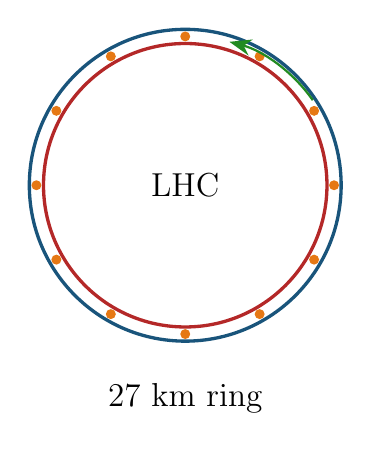
\begin{tikzpicture}[scale=0.9]
                % LHC ring schematic
                \draw[very thick, chaosblue] (0,0) circle (2.2cm);
                \draw[very thick, attractorred] (0,0) circle (2.0cm);
                % Beam particles
                \foreach \a in {0,30,...,330} {
                    \fill[caborange] ({2.1*cos(\a)},{2.1*sin(\a)}) circle (2pt);
                }
                % Labels
                \node at (0,0) {\large LHC};
                \node at (0,-3) {\large 27 km ring};
                % Arrows for motion
                \draw[-{Stealth[scale=1.2]},thick,limitgreen] (1.8,1.2) arc (35:75:2.1);
            \end{tikzpicture}
            
            \vspace{0.5em}
            \large At 6.5 TeV, tiny errors grow \textbf{exponentially}
        \end{column}
    \end{columns}
\end{frame}

\begin{frame}{Particle Dynamics as a Nonlinear Map}
    \begin{block}{\Large One-Turn Map (Symplectic)}
        \[
            \Large
            \begin{pmatrix} x_{n+1} \\ p_{n+1} \end{pmatrix} = 
            \underbrace{\begin{pmatrix} \cos(2\pi Q) & \sin(2\pi Q) \\ -\sin(2\pi Q) & \cos(2\pi Q) \end{pmatrix}}_{\text{Linear rotation}}
            \begin{pmatrix} x_n \\ p_n \end{pmatrix} + 
            \underbrace{\begin{pmatrix} 0 \\ K_2 x_n^2 + \cdots \end{pmatrix}}_{\text{Nonlinear kicks}}
        \]
    \end{block}
    
    \vspace{1em}
    \large
    \begin{itemize}
        \item $Q \approx 64.31$: \textbf{Betatron tune} (oscillations per turn)
        \item $K_2, K_3$: Sextupole, octupole strengths
        \item This is essentially the \textcolor{attractorred}{\textbf{Hénon map}}!
    \end{itemize}
    
    \vspace{0.8em}
    \begin{alertblock}{\large Result}
        Resonance islands, chaotic seas, and a \textbf{dynamic aperture boundary}
    \end{alertblock}
\end{frame}

\begin{frame}{The OGY Method: Taming Chaos}
    \begin{block}{\Large Key Insight (Ott, Grebogi, Yorke 1990)}
        Chaotic systems contain \textbf{infinitely many unstable periodic orbits}. \\
        With \textit{tiny, well-timed perturbations}, you can stabilize any of them!
    \end{block}
    
    \vspace{1em}
    \textbf{\large Near an unstable fixed point:}
    \[
        \Large \delta \mathbf{x}_{n+1} = \mathbf{J} \cdot \delta \mathbf{x}_n
    \]
    
    \vspace{0.5em}
    \large
    Eigenvalues: $|\lambda_s| < 1$ (stable) and $|\lambda_u| > 1$ (unstable)
    
    \vspace{1em}
    \textbf{\large Control law:}
    \[
        \Large \boxed{\delta p = -\frac{\mathbf{g}^T \cdot (\mathbf{x}_n - \mathbf{x}^*)}{|\lambda_u| - 1}}
    \]
    
    \vspace{0.5em}
    Push trajectory onto the \textcolor{limitgreen}{\textbf{stable manifold}} with minimal effort!
\end{frame}

\begin{frame}{LHC Transverse Damper (ADT)}
    \begin{columns}
        \begin{column}{0.55\textwidth}
            \textbf{\large The Feedback Loop:}
            
            \vspace{0.8em}
            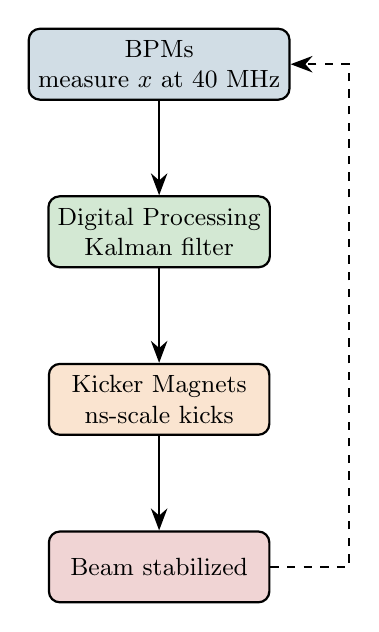
\begin{tikzpicture}[
                node distance=1.2cm,
                box/.style={rectangle, draw, rounded corners, minimum width=2.8cm, minimum height=0.9cm, align=center, font=\small, thick}
            ]
                \node[box, fill=chaosblue!20] (bpm) {BPMs\\measure $x$ at 40 MHz};
                \node[box, fill=limitgreen!20, below=of bpm] (dsp) {Digital Processing\\Kalman filter};
                \node[box, fill=caborange!20, below=of dsp] (kick) {Kicker Magnets\\ns-scale kicks};
                \node[box, fill=attractorred!20, below=of kick] (beam) {Beam stabilized};
                
                \draw[-{Stealth[scale=1.2]},thick] (bpm) -- (dsp);
                \draw[-{Stealth[scale=1.2]},thick] (dsp) -- (kick);
                \draw[-{Stealth[scale=1.2]},thick] (kick) -- (beam);
                \draw[-{Stealth[scale=1.2]},thick,dashed] (beam.east) -- ++(1,0) |- (bpm.east);
            \end{tikzpicture}
        \end{column}
        \begin{column}{0.45\textwidth}
            \textbf{\large Performance Numbers:}
            
            \vspace{0.8em}
            \large
            \begin{tabular}{ll}
                \toprule
                Energy & 6.5 TeV \\
                Protons/bunch & $\sim 10^{11}$ \\
                Bunches & 2,556 \\
                Rev. freq. & 11.245 kHz \\
                ADT bandwidth & 20 MHz \\
                Damping time & 50-100 turns \\
                \bottomrule
            \end{tabular}
            
            \vspace{1em}
            \textcolor{attractorred}{\textbf{Without feedback:}} \\
            Particles hit beam pipe in \textbf{seconds}!
        \end{column}
    \end{columns}
\end{frame}

\begin{frame}{Dynamic Aperture: Order vs Chaos Boundary}
    \begin{columns}
        \begin{column}{0.5\textwidth}
            \textbf{\large Dynamic Aperture (DA):}
            
            \vspace{0.8em}
            The region in phase space where particles remain stable for long times.
            
            \vspace{1em}
            \large
            \begin{itemize}
                \item \textcolor{chaosblue}{\textbf{Inside DA}}: Stable KAM tori
                \item \textcolor{caborange}{\textbf{Boundary}}: Fractal structure
                \item \textcolor{attractorred}{\textbf{Outside DA}}: Chaotic diffusion → loss
            \end{itemize}
            
            \vspace{1em}
            \textbf{LHC requirement:}
            \begin{itemize}
                \item Injection: DA $> 10\sigma$
                \item Collision: DA $> 6\sigma$
            \end{itemize}
        \end{column}
        \begin{column}{0.5\textwidth}
            \centering
            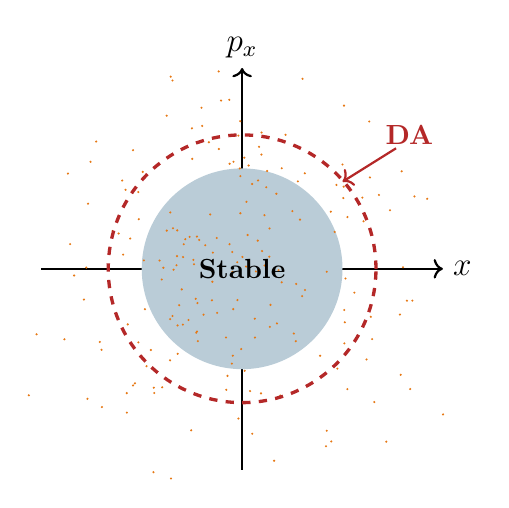
\begin{tikzpicture}[scale=0.85]
                \draw[->,thick] (-3,0) -- (3,0) node[right] {\large $x$};
                \draw[->,thick] (0,-3) -- (0,3) node[above] {\large $p_x$};
                
                % Stable region (blue)
                \fill[chaosblue!30] (0,0) circle (1.5cm);
                
                % Chaotic boundary (orange dots)
                \foreach \i in {1,...,200} {
                    \fill[caborange] ({1.5*rand + 1.8*rand},{1.5*rand + 1.8*rand}) circle (0.5pt);
                }
                
                % DA boundary
                \draw[very thick, attractorred, dashed] (0,0) circle (2cm);
                
                % Labels
                \node at (0,0) {\textbf{Stable}};
                \node[attractorred] at (2.5,2) {\textbf{DA}};
                \draw[->,attractorred,thick] (2.3,1.8) -- (1.5,1.3);
            \end{tikzpicture}
            
            \vspace{0.5em}
            \large Phase space survival map
        \end{column}
    \end{columns}
\end{frame}

\begin{frame}{Theory Meets Practice: Summary}
    \begin{center}
    \large
    \begin{tabular}{l|l}
        \toprule
        \textbf{Chaos Theory} & \textbf{CERN Application} \\
        \midrule
        Phase space & Track $(x, p_x, y, p_y, z, \delta)$ \\
        Strange attractor & Beam halo \\
        Unstable fixed point & Design orbit \\
        Sensitive dependence & Injection errors amplify \\
        Lyapunov exponent & Tune stability margins \\
        Poincaré section & Turn-by-turn BPM data \\
        OGY control & Transverse damper \\
        Dynamic aperture & Machine protection \\
        \bottomrule
    \end{tabular}
    \end{center}
    
    \vspace{1em}
    \begin{exampleblock}{\large Key Message}
        Everything we learned about chaos theory is \textbf{applied daily} at CERN to keep $10^{14}$ protons on track at 99.9999991\% the speed of light!
    \end{exampleblock}
\end{frame}

%=============================================================================
% CONCLUSION
%=============================================================================
\section{Conclusion}

\begin{frame}{Summary: From Limit Cycles to Chaos Control}
    \begin{columns}
        \begin{column}{0.33\textwidth}
            \centering
            \textcolor{limitgreen}{\textbf{\Large Limit Cycles}}
            
            \vspace{0.8em}
            \begin{itemize}
                \item Periodic, predictable
                \item Van der Pol oscillator
                \item Heartbeat modeling
                \item $\lambda_{\max} = 0$
            \end{itemize}
        \end{column}
        \begin{column}{0.33\textwidth}
            \centering
            \textcolor{attractorred}{\textbf{\Large Strange Attractors}}
            
            \vspace{0.8em}
            \begin{itemize}
                \item Aperiodic, chaotic
                \item Lorenz system
                \item Fractal geometry
                \item $\lambda_{\max} > 0$
            \end{itemize}
        \end{column}
        \begin{column}{0.33\textwidth}
            \centering
            \textcolor{chaosblue}{\textbf{\Large Chaos Control}}
            
            \vspace{0.8em}
            \begin{itemize}
                \item OGY method
                \item Tiny perturbations
                \item CERN beam control
                \item Stabilize UPOs
            \end{itemize}
        \end{column}
    \end{columns}
    
    \vspace{1.5em}
    \begin{alertblock}{\large Key Takeaway}
        Deterministic systems can exhibit unpredictable behavior—but \textbf{chaos can be controlled} with the right mathematical tools!
    \end{alertblock}
\end{frame}

\begin{frame}{Key Equations Cheat Sheet}
    \Large
    \textbf{Van der Pol:}
    \[
        \ddot{x} - \mu(1-x^2)\dot{x} + x = 0
    \]
    
    \textbf{Lorenz:}
    \[
        \dot{x} = \sigma(y-x), \quad \dot{y} = x(\rho-z) - y, \quad \dot{z} = xy - \beta z
    \]
    
    \textbf{Lyapunov Exponent:}
    \[
        |\delta \mathbf{x}(t)| \sim |\delta \mathbf{x}_0| e^{\lambda t}
    \]
    
    \textbf{OGY Control:}
    \[
        \delta p = -\frac{\mathbf{g}^T \cdot (\mathbf{x}_n - \mathbf{x}^*)}{|\lambda_u| - 1}
    \]
\end{frame}

\begin{frame}{Further Reading}
    \large
    \begin{thebibliography}{9}
        \bibitem{strogatz} S.H. Strogatz, \textit{Nonlinear Dynamics and Chaos}, Westview Press, 2015.
        \bibitem{lorenz} E.N. Lorenz, ``Deterministic Nonperiodic Flow,'' \textit{J. Atmos. Sci.} \textbf{20}, 130--141 (1963).
        \bibitem{ogy} E. Ott, C. Grebogi, J.A. Yorke, ``Controlling Chaos,'' \textit{Phys. Rev. Lett.} \textbf{64}, 1196 (1990).
        \bibitem{feigenbaum} M.J. Feigenbaum, ``Quantitative Universality...'' \textit{J. Stat. Phys.} \textbf{19}, 25--52 (1978).
        \bibitem{wiedemann} H. Wiedemann, \textit{Particle Accelerator Physics}, Springer, 2015.
    \end{thebibliography}
\end{frame}

\begin{frame}
    \centering
    \Huge\textcolor{chaosblue}{Thank You}
    
    \vspace{1.5em}
    \Large Questions?
    
    \vspace{2.5em}
    \large
    \textit{``The universe is not only queerer than we suppose,\\
    but queerer than we can suppose.''}\\[0.5em]
    — J.B.S. Haldane
    
    \vspace{1em}
    \normalsize
    \textcolor{limitgreen}{\textit{At CERN, we've learned to harness that queerness.}}
\end{frame}

\end{document}
